\section{Models and different Approaches}

\subsection{DQN Introduction}

Model-free based Deep Q Network algorithm was chosen specifically for the state size and complexity. DQN builds off of Q-learning algorithms by using a Deep Neural Network (DNN) for approximating the state-action value function, Q(s, a). Function Q(s, a) is defined such that for given state $s$ and action $a$ it returns an estimate of a total reward we would achieve starting at this state, taking the action and then following some policy. Let’s call the Q function for the optimal policies $Q_{opt}$.
 $Q_{opt}$ with discounting can be written as 
 \begin{equation}
Q_{opt}(s,a) = r_{0} + \gamma r_{1} + \gamma^{2} r_{2} + ...
\end{equation}
Here, $r$ stands for rewards. $\gamma$ is called a discount factor and when set it to $\gamma < $  1 , it makes sure that the sum in the formula is finite. The $\gamma$ controls how much the function Q in state $s$ depends on the future and so it can be thought of as how much ahead the agent sees.  \newline
The above equation can be rewritten in a recursive form.
 \begin{equation}
Q_{opt}(s,a) = r_{0} + \gamma max_{a}Q_{opt}(s',a)
\end{equation}
This equation is proven to converge to the desired $Q_{opt}$, with finite number of states and each of the state-action pair is presented repeatedly. However, the Lunar Lander state space is real and continuous. We cannot store infinite number of values for every possible state. Instead, we  approximate the Q function with a neural network. This network will take a state as an input and produce an estimation of the Q function for each action. This network with multiple layers is called Deep Q-network (DQN).
\newline \newline
\textbf{Experience Replay} \newline \newline
During each simulation step, the agent perform an action $a$ in state $s$, receives immediate reward $r$ and come to a new state $s’$.
\newline
There are two problems with online learning - \newline
1. The samples arrive in order they are experienced and as such are highly correlated. This might cause overfitting.
\newline
2. Throwing away each sample immediately after we use it. This means we are not using our experience effectively.
\newline
The key idea of 'experience replay' is that we store these $(s, a, r, s')$ transitions in a memory and during each learning step, sample a random batch and perform a gradient descend on it. This way we solve both issues.
After reaching the finite allotted memory capacity, the oldest sample is discarded.
\newline \newline
\textbf{Exploration}
To find out that actions which might be better then others, we use $\epsilon$ greedy policy. This policy behaves greedily most of the time, but chooses a random action with probability $\epsilon$. $\epsilon$ will be a hyper-parameter played with to make sure our agent learns fast enough while consistently performing better.

\subsection{Full DQN}
In DQN algorithm we set targets for gradient descend as:
\begin{equation}
Q_{opt}(s,a) = r_{0} + \gamma max_{a}Q_{opt}(s',a)
\end{equation}
We see that the target depends on the current network. A neural network works as a whole, and so each update to a point in the Q function also influences whole area around that point. And the points of $Q(s, a)$ and $Q(s’, a)$ are very close together, because each sample describes a transition from $s$ to $s’$. This leads to a problem that with each update, the target is likely to shift. This can lead to instabilities, oscillations or divergence.
\newline
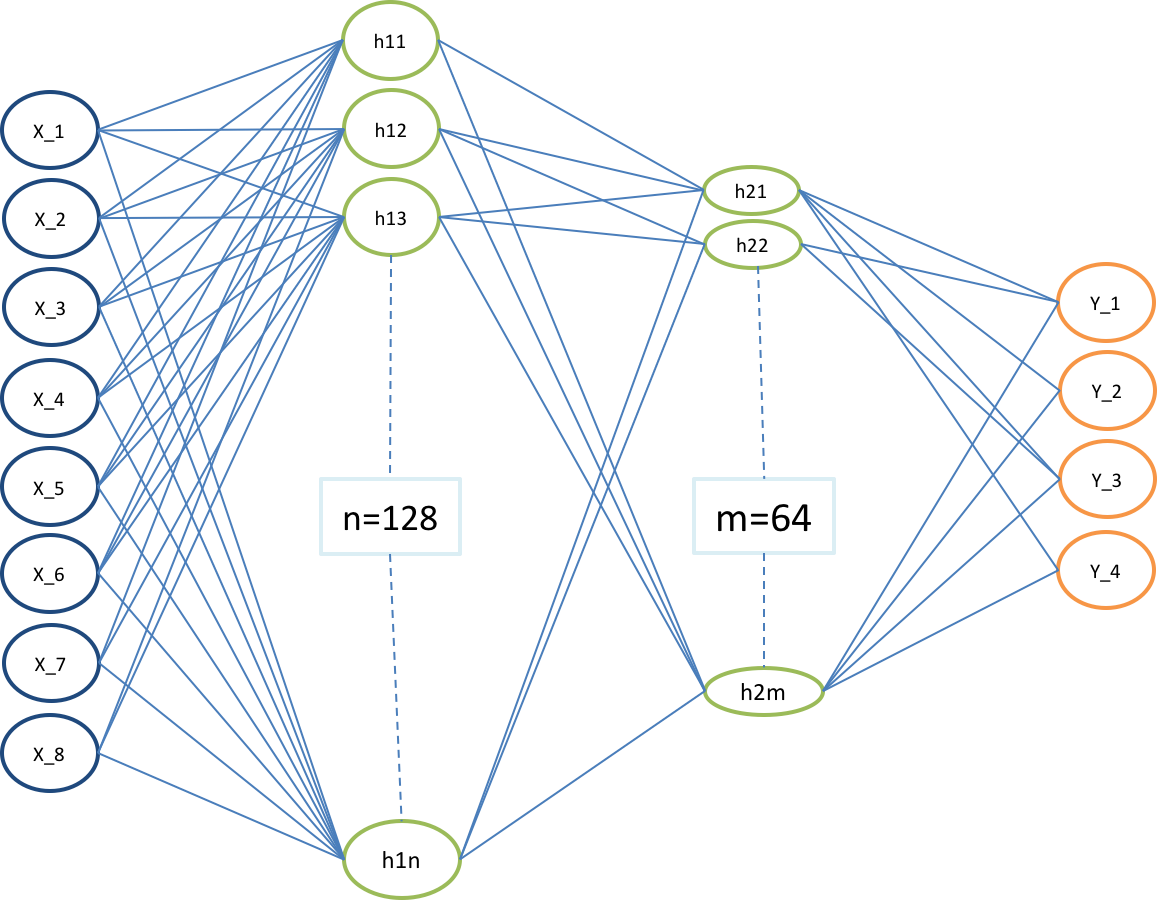
\includegraphics[scale=0.75,width=0.75\columnwidth]{figures/NN.png}%
\newline
To overcome this problem, researches proposed to use a separate target network for setting the targets. This network is a mere copy of the previous network, but frozen in time. It provides stable $\tilde{Q}$ values and allows the algorithm to converge to the specified target:
\begin{equation}
Q(s, a) \xrightarrow{} r + \gamma max_a \tilde{Q}(s', a)
\end{equation}

After several steps, the target network is updated, just by copying the weights from the current network. To be effective, the interval between updates has to be large enough to leave enough time for the original network to converge. \newline
For lunar lander, we update target model after every episode.

\subsection{Double DQN}
One problem in the DQN algorithm is that the agent tends to overestimate the Q function value, due to the max in the formula used to set targets.
Because of the max in the formula, the action with the highest positive/negative error could be selected and this value might subsequently propagate further to other states. This leads to bias – value overestimation. This severe impact on stability of the learning algorithm.
\newline
In this new algorithm, two Q functions $Q_{1}$ and $Q_2$ – are independently learned. One function is then used to determine the maximizing action and second to estimate its value. Either $Q_1$ or $Q_2$ is updated randomly with a formula:
\begin{equation}
Q_1(s, a) \xrightarrow{} r + \gamma Q_2(s', argmax_a Q_1(s', a)) 
\end{equation}
or
\begin{equation}
Q_2(s, a) \xrightarrow{} r + \gamma Q_1(s', argmax_a Q_2(s', a)) 
\end{equation}
It was proven that by decoupling the maximizing action from its value in this way, one can indeed eliminate the maximization bias.
\newline
When thinking about implementation into the DQN algorithm, we can leverage the fact that we already have two different networks giving us two different estimates Q and $\tilde{Q}$ (target network). Although not really independent, it allows us to change our algorithm in a really simple way.
\newline
The original target formula would change to:
\begin{equation}
Q(s, a) \xrightarrow{} r + \gamma \tilde{Q}(s', argmax_a Q(s', a))
\end{equation}
We could observe that Double DQN was more stable than Full DQN.
 
\subsection{Dueling layer DQN}
Q(s,a) represents the value of a given action $a$ chosen in state $s$, V(s) represents the value of the state independent of action. By definition, $V(s)=max_{a}Q(s,a)$. Thus, A(s,a) provides a relative measure of the utility of actions in s. The insight behind the dueling network architecture is that sometimes the exact choice of action does not matter so much, and so the state could be more explicitly modeled, independent of the action. There are two neural networks — one learns to provide an estimate of the value at every timestep, and the other calculates potential advantages of each action, and the two are combined for a single action-advantage Q function. We can achieve more robust estimates of state value by decoupling it from the necessity of being attached to specific actions.
 [FIXME https://arxiv.org/pdf/1511.06581.pdf]
\newline
\begin{equation}
Q(s,a) \rightarrow A(s,a) + V(s)
\end{equation}
The above equation is unidentifiable in the sense that given $Q$
we cannot recover $V$ and $A$ uniquely. This lack of identifiability is mirrored by poor practical performance when this equation is used directly. To address this issue of identifiability, we can force the advantage
function estimator to have zero advantage at the
chosen action. That is, we let the last module of the network
implement the forward mapping.
\begin{equation}
Q(s,a; \theta, \alpha, \beta) \rightarrow V(s; \theta, \beta) + (A(s,a\theta, \alpha) - max_{a' \epsilon |A|} A(s,a';\theta,\alpha ))
\end{equation}
An alternative module replaces the max operator with an
average. On the one hand this loses the original semantics of V and
A because they are now off-target by a constant, but on
the other hand it increases the stability of the optimization:
with this following equation-
\begin{equation}
Q(s,a; \theta, \alpha, \beta) \rightarrow V(s; \theta, \beta) + (A(s,a\theta, \alpha) - \frac{1}{A} \sum_{a'}^{} A(s,a';\theta,\alpha ))
\end{equation}
 the advantages (A) only need to change as fast as the
mean, instead of having to compensate any change to the
optimal action’s advantage in  (13)
\newline
 \textcolor{red}{\texttt{ Good to draw the neural network used by use for DUELDQN, something similar to figure1 of https://arxiv.org/pdf/1511.06581.pdf }}
